\chapter{Manual de Configuración del Plugin}
\label{Appendix:Configuracion}

Este apéndice describe detalladamente cada uno de los parámetros configurables del plugin \textit{obs-domjudge-ar-overlay} a través del panel de propiedades nativo de OBS Studio. Para acceder a dicha interfaz, el usuario debe hacer clic derecho sobre la fuente de vídeo correspondiente en el panel de fuentes, seleccionar la opción \textit{Filtros} en el menú contextual y, finalmente, hacer clic sobre el filtro asignado al plugin.

El selector principal de la interfaz es el menú desplegable \textbf{Modo de renderizado}. Este componente actúa como un conmutador dinámico que reestructura la interfaz gráfica de usuario, mostrando u ocultando los paneles de control específicos según el modo de operación seleccionado. Los cinco modos disponibles se detallan a continuación: \textbf{3D}, \textbf{AR}, \textbf{Countdown (Reloj)}, \textbf{Scoreboard (Texto)} y \textbf{Team Info}.

% =======================================================
\section{Modo 3D (Renderizado Fijo)}
\label{sec:modo-3d}

Este modo permite renderizar un modelo tridimensional en una posición estática y absoluta dentro del lienzo de la escena de OBS Studio, prescindiendo por completo de los algoritmos de visión artificial y de la detección de marcadores. Su configuración se divide en el ajuste espacial del objeto y la carga de activos digitales:

\begin{itemize}
    \item \textbf{Posición X / Y / Z:} Define las coordenadas espaciales del centro del modelo dentro del espacio tridimensional proyectado en la pantalla. Admite un rango de valores de $[ -3000, 3000 ]$.
    \item \textbf{Escala:} Aplica un factor de escala uniforme sobre los tres ejes del modelo geométrico para adaptar su tamaño al lienzo. Admite un rango paramétrico de $[ 0.1, 1000.0 ]$.
    \item \textbf{Rotación X / Y / Z (Grados):} Controla la orientación angular del objeto respecto a los ejes de coordenadas del mundo virtual. El rango operativo abarca desde $-360^\circ$ hasta $360^\circ$.
    \item \textbf{Ruta del Modelo 3D:} Ruta absoluta en el sistema de archivos local hacia el archivo geométrico que se desea instanciar. El motor del plugin es compatible con los formatos estándar \texttt{.obj}, \texttt{.fbx}, \texttt{.dae} y \texttt{.gltf}.
    \item \textbf{Ruta de la Textura:} Especifica el mapa de bits que se aplicará sobre la envoltura (malla) del modelo 3D para definir su apariencia superficial. Soporta archivos en formato \texttt{.png}, \texttt{.jpg} y \texttt{.bmp}.
\end{itemize}

\begin{figure}[H]
    \centering
    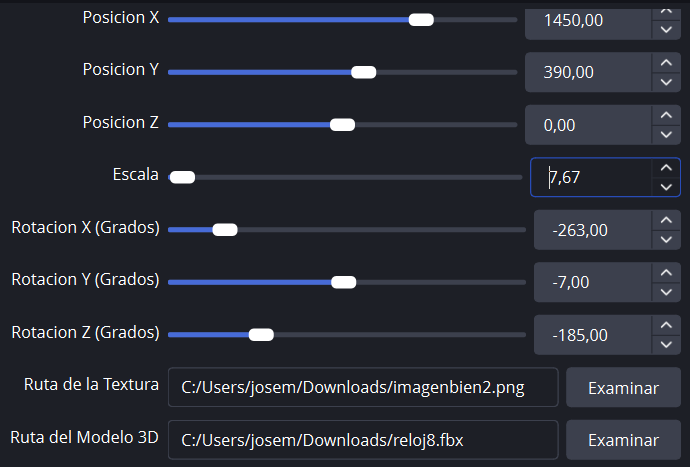
\includegraphics[width=0.9\textwidth]{Imagenes/Vectorial/UI_modo3D.png}
    \caption{Interfaz de usuario del plugin configurada en el Modo 3D.}
    \label{fig:ui-modo-3d}
\end{figure}

% =======================================================
\section{Modo AR (Realidad Aumentada sobre Marcador Único)}
\label{sec:modo-ar}

El Modo AR activa el hilo de procesamiento de visión artificial. Su propósito es detectar en tiempo real un marcador ArUco en el flujo de vídeo para anclar el modelo 3D sobre él de forma dinámica. En esta modalidad, los controles de posicionamiento manual quedan deshabilitados, delegando el cálculo de coordenadas espaciales al motor de estimación de pose.

\subsection{Configuración del Modelo 3D}
Los parámetros relativos a la carga del objeto geométrico (\textbf{Ruta del Modelo 3D} y \textbf{Ruta de la Textura}) mantienen el mismo comportamiento analizado en el modo estático (Sección~\ref{sec:modo-3d}). Se preserva la variable \textbf{Escala} ($[ 0.1, 1000.0 ]$) como un factor multiplicador para normalizar el tamaño del objeto importado.

\subsection{Parámetros de Detección ArUco}
Este panel parametriza el comportamiento de los algoritmos de detección de OpenCV:

\begin{itemize}
    \item \textbf{ID del Marker:} Identificador numérico correlativo asignado al marcador que el plugin debe buscar en la imagen. Admite un rango entero de $[ 0, 100 ]$ y debe coincidir exactamente con el patrón del marcador impreso.
    \item \textbf{Tamaño del Marker:} Especifica la longitud real del lado del marcador físico (expresada en unidades métricas o escala de referencia). Su rango varía de $[ 0.1, 10.0 ]$. Configurar un valor erróneo puede alterar de manera directamente proporcional el cálculo de la distancia (eje Z) y la escala del modelo.
    \item \textbf{Diccionario de Marker:} Selector de la familia o diccionario de generación de marcadores ArUco. El sistema ofrece compatibilidad con las siguientes distribuciones: \texttt{Original}, \texttt{4x4 (100)}, \texttt{5x5 (100)}, \texttt{6x6 (100)} y \texttt{7x7 (100)}.
    \item \textbf{Archivo de Calibración:} Almacena la ruta local hacia el fichero de configuración en formato \texttt{.yml}. Este archivo contiene la matriz de la cámara y los coeficientes de distorsión intrínseca obtenidos previamente mediante el asistente de calibración del plugin. Si se omite, el sistema aplica una matriz identidad genérica por defecto, lo que puede provocar desfases y distorsiones ópticas en el posicionamiento del modelo.
\end{itemize}

\begin{figure}[H]
    \centering
    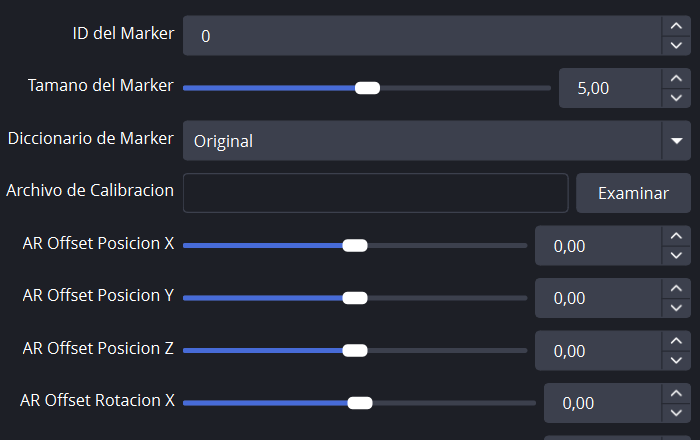
\includegraphics[width=0.9\textwidth]{Imagenes/Vectorial/UI_modo3DAR.png}
    \caption{Interfaz de usuario del plugin configurada en el Modo AR.}
    \label{fig:ui-modo-ar}
\end{figure}

\subsection{Ajustes de Posicionamiento Relativo (Offsets)}
Diseñados para corregir pequeñas desviaciones métricas producidas por tolerancias en la impresión física o imprecisiones en la calibración de la lente sin necesidad de reiniciar el proceso:

\begin{itemize}
    \item \textbf{AR Offset Posición X / Y / Z:} Desplazamiento lineal del origen del modelo 3D respecto al centro geométrico del marcador detectado (rango operativo de $[ -1000, 1000 ]$).
    \item \textbf{AR Offset Rotación X / Y / Z:} Corrección angular fina (expresada en grados de $-360^\circ$ a $360^\circ$) aplicada sobre los ejes locales del marcador.
\end{itemize}

\begin{figure}[H]
    \centering
    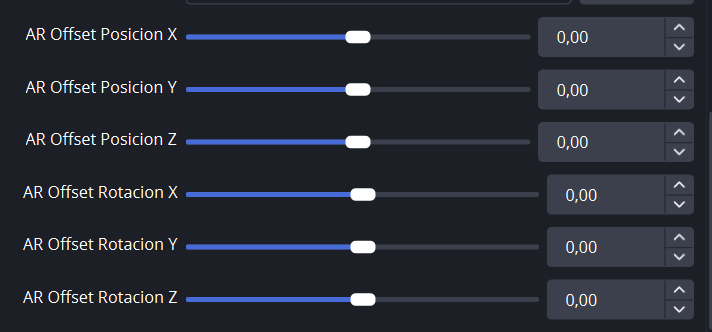
\includegraphics[width=0.9\textwidth]{Imagenes/Vectorial/modooffsets.png}
    \caption{Panel de control de offsets de posicionamiento en el Modo AR.}
    \label{fig:ui-ar-offsets}
\end{figure}

% =======================================================
\section{Módulo de Conexión y Sincronización con DOMjudge}
\label{sec:conexion-domjudge}

Los modos de visualización de datos (\textbf{Countdown}, \textbf{Scoreboard} y \textbf{Team Info}) requieren la extracción de información estructurada en tiempo real desde la plataforma de arbitraje competitivo DOMjudge. El panel encargado de gestionar el intercambio de peticiones a través de la API REST es idéntico para los tres modos y expone las siguientes directivas:

\begin{itemize}
    \item \textbf{Sincronizar con DOMjudge (Sincronización Web):} Interruptor booleano que activa o desactiva el subproceso (\textit{thread}) encargado de realizar las peticiones HTTP GET periódicas a la API.
    \item \textbf{URL API (DOMjudge):} Dirección URL base del punto de acceso de la API de la instancia activa de DOMjudge.
    
    (por ejemplo, \texttt{https://miservidor.domjudge.org/api/v4}). Se debe evitar la inclusión de una barra diagonal inversa (\texttt{/}) al final de la cadena de texto. Este campo es crítico y específico para cada evento competitivo.
    \item \textbf{Contest ID:} Identificador único numérico del concurso que se desea monitorizar. Este valor puede localizarse directamente inspeccionando la URL de la interfaz de administración web de DOMjudge.
    \item \textbf{Usuario API / Contraseña API:} Credenciales de autenticación HTTP Basic asociadas a un perfil de usuario con permisos de lectura válidos dentro de la plataforma DOMjudge. El campo de la contraseña enmascara los caracteres por motivos de seguridad.
    \item \textbf{Probar Conexión:} Botón de acción asíncrona que despacha una petición de prueba a la API. El código de respuesta HTTP y el estado del enlace de red son redirigidos directamente al registro interno de OBS Studio (\textit{Ayuda} $\rightarrow$ \textit{Archivos de registro} $\rightarrow$ \textit{Ver registro actual}).
    \item \textbf{Intervalo Sinc (seg) / Intervalo API (seg):} Define el periodo de refresco de la tarea automatizada de sincronización (rango de $[ 1, 300 ]$ segundos). Para entornos de producción estándar, se recomienda fijar un umbral de $30$ segundos para mitigar la sobrecarga de peticiones sobre el servidor web.
\end{itemize}

\begin{figure}[H]
    \centering
    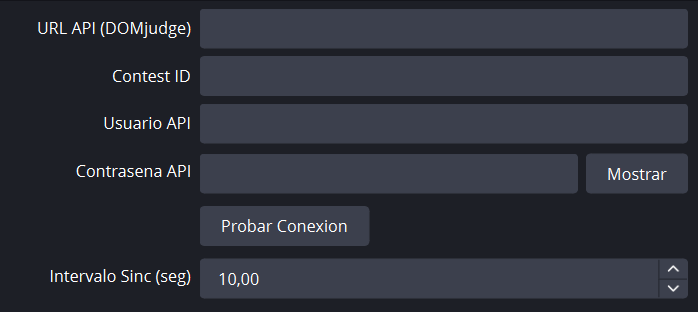
\includegraphics[width=0.9\textwidth]{Imagenes/Vectorial/sincrodomjug.png}
    \caption{Panel común de configuración e integración con la API REST de DOMjudge.}
    \label{fig:ui-sincro-domjudge}
\end{figure}

% =======================================================
\section{Modo Countdown (Reloj Analógico)}
\label{sec:modo-countdown}

Este modo asocia los tiempos de duración del concurso (extraídos desde el módulo de sincronización descrito en la Sección~\ref{sec:conexion-domjudge}) a las mallas de un reloj analógico tridimensional que actúa como cuenta atrás visual en la transmisión.

\subsection{Modelo 3D y Posicionamiento Dinámico}
Los bloques de selección de rutas de modelos 3D y mapas de texturas replican fielmente la lógica anterior. La principal diferencia radica en el método de proyección, el cual es gobernado por una directiva dedicada:

\begin{itemize}
    \item \textbf{Reloj en Marker AR:} Actúa como un conmutador. Si se encuentra \textbf{desactivado}, el reloj se renderiza usando las variables estáticas (\textbf{Posición} y \textbf{Rotación X/Y/Z}) descritas en la Sección~\ref{sec:modo-3d}. Si se encuentra \textbf{activado}, la interfaz oculta de forma dinámica los controles manuales para evitar la sobrecarga visual y el objeto se ancla al marcador  definido en los parámetros globales del Modo AR (Sección~\ref{sec:modo-ar}).
\end{itemize}

\subsection{Configuración de la Cuenta Atrás y Animación}
\begin{itemize}
    \item \textbf{Cuenta Atrás:} Activa la rutina matemática que decrementa temporalmente el estado del concurso en función del reloj del sistema.
    \item \textbf{Reiniciar Reloj:} Fuerza la inicialización del temporizador interno al valor del tiempo inicial estipulado en la configuración del concurso.
    \item \textbf{Manecillas Reloj:} Menú de selección que define el algoritmo de rotación y animación de los sub-componentes (nodos de la malla) del modelo cargado:
    \begin{itemize}
        \item \textbf{H/M/S (3):} Modo tri-axial independiente. El nodo asignado a la manecilla de los segundos efectúa un barrido discreto  por segundo; el nodo de los minutos progresa  por cada minuto transcurrido, y el nodo de las horas se desplaza proporcionalmente al intervalo de tiempo transcurrido del evento.
        \item \textbf{Total (1):} Modo unificado de progreso. El plugin selecciona una única aguja o componente del modelo y calcula una rotación lineal de $360^\circ$ mapeada sobre la duración total del concurso.
    \end{itemize}
\end{itemize}

\begin{figure}[H]
    \centering
    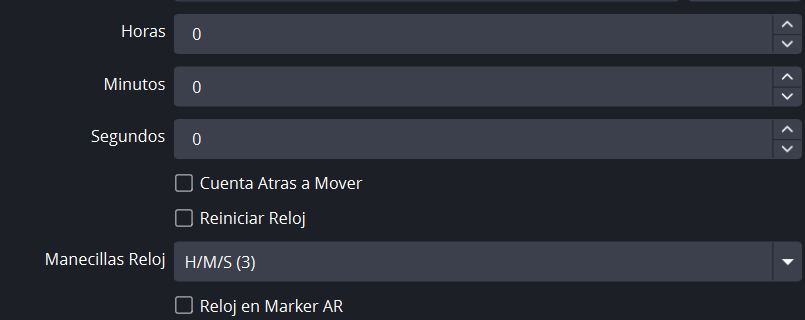
\includegraphics[width=0.9\textwidth]{Imagenes/Vectorial/modocountdown.png}
    \caption{Interfaz de usuario del plugin configurada en el Modo Countdown.}
    \label{fig:ui-modo-countdown}
\end{figure}

% =======================================================
\section{Modo Scoreboard (Superposición de Texto Bidimensional)}
\label{sec:modo-scoreboard}

El Modo Scoreboard transforma los datos de la clasificación general obtenidos de DOMjudge en un componente de texto bidimensional avanzado superpuesto sobre la señal de vídeo.

\subsection{Posicionamiento del Componente Gráfico}
\begin{itemize}
    \item \textbf{Anclar al marcador AR:} Vincula el origen del marcador ArUco a la visualización de la clasificación, permitiendo que la tabla siga el movimiento físico del objetivo en el plano de la cámara.
    \item \textbf{Centrar en Pantalla:} Directiva booleana que calcula la resolución nativa de la fuente de vídeo para posicionar el lienzo del \textit{scoreboard} simétricamente en el baricentro de la escena, invalidando los campos de control manual.
    \item \textbf{Offset Manual X / Y:} Desplazamiento en píxeles aplicado en el espacio de coordenadas bidimensional del lienzo cuando la opción de centrado automático se encuentra inactiva (rango operativo de $[ 0, 3000 ]$).
\end{itemize}

\subsection{Estilo y Apariencia del Texto}
Este conjunto de parámetros permite homogeneizar el componente gráfico con la línea de diseño corporativo de DOMjudge:
\begin{itemize}
    \item \textbf{Tamaño de Fuente:} Escala en puntos del tamaño tipográfico (rango de $[ 5, 150 ]$).
    \item \textbf{Color del Texto / Color del Borde:} Selectores de color en formato RGBA que definen el cuerpo del carácter y su contorno decorativo.
    \item \textbf{Grosor del Borde:} Espesor en píxeles asignado al perfilado de la tipografía (rango de $[ 0, 20 ]$).
    \item \textbf{Max caracteres equipo:} Ajuste de seguridad contra desbordamientos visuales. Aplica una función de truncado con puntos suspensivos sobre aquellos nombres de equipos que excedan el límite de caracteres configurado ($[ 5, 40 ]$).
    \item \textbf{Bandas por fila / Opacidad bandas (\%):} Activa una técnica de renderizado que alterna el sombreado de fondo entre filas pares e impares, emulando la interfaz web original de DOMjudge para mejorar la legibilidad. Admite un ajuste de opacidad de $[ 0, 80 ]\%$.
\end{itemize}

\subsection{Fondo del Overlay}
\begin{itemize}
    \item \textbf{Activar fondo del texto:} Habilita la composición de una caja o rectángulo delimitador detrás de la matriz de texto.
    \item \textbf{Color de fondo / Opacidad fondo (\%):} Establece las propiedades cromáticas y el nivel de transparencia del plano delimitador ($[ 0, 100 ]\%$).
    \item \textbf{Margen interno (px):} Distancia de separación (\textit{padding}) entre los extremos del texto y los bordes limítrofes del contenedor rectangular (rango de $[ 0, 80 ]$).
    \item \textbf{Radio esquinas (px):} Configura el redondeo geométrico de los vértices del rectángulo mediante curvas de Bézier (rango de $[ 0, 80 ]$).
\end{itemize}

\subsection{Sombra del Overlay}
\begin{itemize}
    \item \textbf{Activar sombra:} Renderiza un efecto de proyección de sombra paralela para separar visualmente el overlay del flujo de vídeo de fondo.
    \item \textbf{Opacidad sombra (\%):} Nivel de transparencia de la sombra ($[ 0, 100 ]\%$).
    \item \textbf{Sombra offset X / Y (px):} Vector de desplazamiento bidimensional del sombreado ($[ -50, 50 ]$).
    \item \textbf{Sombra suavidad (capas):} Número de pasadas consecutivas ejecutadas por el algoritmo de desenfoque. Valores altos incrementan la suavidad visual a costa de mayor carga computacional en la GPU (rango de $[ 1, 8 ]$).
\end{itemize}

\subsection{Suavizado de Posición AR}
Filtros aplicados para mitigar el ruido de alta frecuencia y el temblor cinético (*jitter*) propio de las transformaciones estimadas por visión artificial:
\begin{itemize}
    \item \textbf{Suavizado AR (overlay):} Habilita la inserción de un filtro pasa-bajo exponencial en la cadena de actualización posicional.
    \item \textbf{Suavizado AR (alpha):} Factor matemático de ponderación inter-frame (rango numérico de $[ 0.01, 1.0 ]$). Un coeficiente cercano a $1.0$ prioriza la respuesta inmediata ante movimientos bruscos; un coeficiente próximo a $0.01$ atenúa drásticamente el ruido, dotando al overlay de mayor inercia visual y transiciones más homogéneas.
\end{itemize}

\begin{figure}[H]
    \centering
    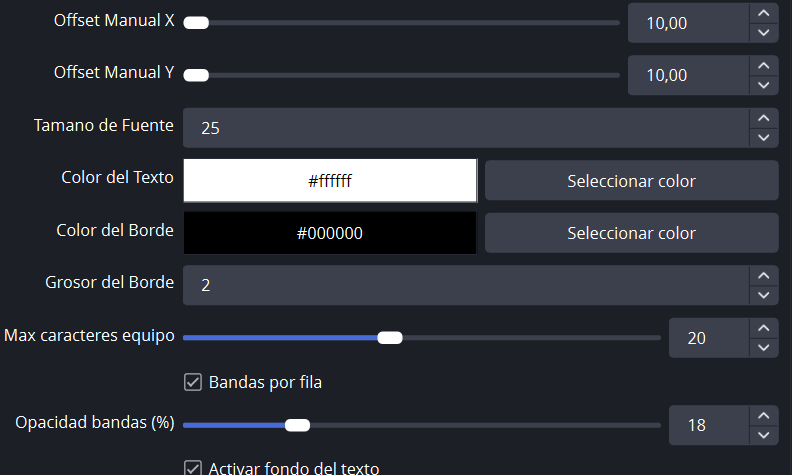
\includegraphics[width=0.9\textwidth]{Imagenes/Vectorial/modoscoreboard1.png}
    \caption{Interfaz de usuario del plugin configurada en el Modo Scoreboard.}
    \label{fig:ui-modo-scoreboard}
\end{figure}

% =======================================================
\section{Modo Team Info (Mapeo Multimarcador)}
\label{sec:modo-team-info}

El Modo Team Info está diseñado para la realización de tomas individuales en las mesas de los competidores. A diferencia del Modo AR básico, esta funcionalidad utiliza un algoritmo de escaneo capaz de reconocer múltiples marcadores registrados en un archivo de configuración local externo y asociarlos dinámicamente a la API de DOMjudge.

Este modo hereda todos los parámetros estéticos, de renderizado, de sombras y filtros de suavizado exponencial analizados en el Modo Scoreboard (Sección~\ref{sec:modo-scoreboard}). Sin embargo, presenta variaciones estructurales en su lógica operativa: carece de centrado automático o controles de posición manual, debido a que el cuadro informativo aparece exclusivamente posicionado sobre el marcador del equipo que esté capturando la cámara en ese instante.

\begin{itemize}
    \item \textbf{Diccionario de Marker:} Familia ArUco asignada de manera unificada para la lectura del conjunto total de marcadores del entorno.
    \item \textbf{JSON de equipos (ArUco$\rightarrow$Team):} Ruta absoluta hacia el archivo de configuración con formato estructurado \texttt{.json} que implementa la base de datos de mapeo. El archivo debe validar el siguiente esquema sintáctico:
\end{itemize}

\begin{verbatim}
        [
          { "marker_id": 1, "team_id": "42" },
          { "marker_id": 2, "team_id": "12" }
        ]
\end{verbatim}

Donde \texttt{marker\_id} representa el identificador numérico de la tarjeta física ArUco dispuesta en el puesto de competición y \texttt{team\_id} es el identificador único del equipo asignado dentro de la plataforma DOMjudge. El búfer interno del plugin está optimizado para procesar un mapeo dinámico de hasta 16 entradas simultáneas.

\begin{itemize}
    \item \textbf{Recargar JSON:} Botón de interrupción que fuerza al plugin a volver a parsear el archivo \texttt{.json} desde el disco local de manera asíncrona. Esto permite actualizar el mapeo de equipos sobre la marcha durante la retransmisión sin necesidad de desactivar el filtro de la escena ni reiniciar OBS Studio.
\end{itemize}

\begin{figure}[H]
    \centering
    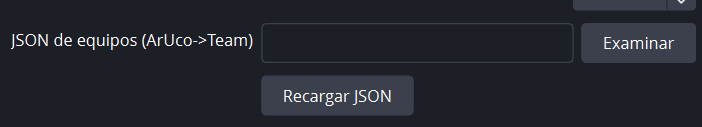
\includegraphics[width=0.9\textwidth]{Imagenes/Vectorial/modoteaminfo.png}
    \caption{Interfaz de usuario del plugin configurada en el Modo Team Info.}
    \label{fig:ui-modo-team-info}
\end{figure}